\documentclass[t,professionalfonts,handout, xcolor=pdftex,dvipsnames,table]{beamer}

\usepackage{pgfpages}
\usepackage{graphics}
\usepackage{graphicx}
\usepackage{amssymb, amsmath}
\usepackage{fancybox}
\usepackage{rotating}
\usepackage{color}

\font\bbb=msbm10
\def \R {\hbox{\bbb R}}
\def \E {\hbox{\bbb E}}
\def \V {\hbox{\bbb V}}
\def \P {\hbox{\bbb P}}
\def \C {\hbox{\bbb C}}

\def\MET{\mbox{${\hbox{$E$\kern-0.6em\lower-.1ex\hbox{/}}}_T$}}
\def\squark{$\tilde{q}$}                 %squark
\def\gluino{$\tilde{g}$}                  %gluino
\def\chipm{$\tilde{\chi}^{\pm}$}   %chi+/-
\def\chiz{$\tilde{\chi}^0$}              %chi0

\def\Journal#1#2#3#4{{#1} {\bf #2}, #3 (#4)}

\newcommand{\Equation}[1]{Equation (\ref{eq:#1})}
\newcommand{\Eq}[1]{Eq.\ (\ref{eq:#1})}
\newcommand{\Eqs}[2]{Eqs.\ (\ref{eq:#1}) and (\ref{eq:#2})}
\newcommand{\Eqns}[3]{Eqs.\ (\ref{eq:#1}), (\ref{eq:#2}) and (\ref{eq:#3})}
\newcommand{\Fig}[1]{Fig.\ \ref{fig:#1}}
\newcommand{\Figs}[2]{Figs.\ \ref{fig:#1} and \ref{fig:#2}}
\newcommand{\Figure}[1]{Figure\ \ref{fig:#1}}
\newcommand{\Figures}[2]{Figures\ \ref{fig:#1} to \ref{fig:#2}}
\newcommand{\Sec}[1]{Sec.~\ref{sec:#1}}

\newcommand{\barR}{\overline{\bf R}}
\newcommand{\prob}[2]{ \mbox{P} (#1 | #2)}
\newcommand{\pdf}[2]{ f (#1 | #2)}
\newcommand{\priorpdf}[1]{ \pi (#1)}
\newcommand{\prior}[1]{ \mbox{P} (#1)}
\newcommand{\like}[1]{ L (#1)}
\newcommand{\flatpri}[1]{\pi_{\rm F}(#1)}
\newcommand{\tab}{aaaaa\=}
\newcommand{\WIDTH}{8.0cm}
\newcommand{\ANGLE}{90}
\newcommand{\SIZE}{0.375\textwidth}

\newcommand{\rlambda}{\textcolor{red}{\lambda}}
\newcommand{\bkappa}{\textcolor{blue}{\kappa}}
\newcommand{\mnu}{\textcolor{magenta}{\nu}}

\usecolortheme[named=Blue]{structure}
\setbeamertemplate{navigation symbols}{}
\setbeamercovered{transparent}

\usetheme{Warsaw}
%\useoutertheme{infolines}
%\usetheme{Madrid}

\title[Contact Interactions]{Search for Contact Interactions using Inclusive Jet Production Cross Sections @ 13\,TeV}
\author[S.Beri, S. Dutt, B. Kotwal, H.B. Prosper]{Suman Beri \inst{1}, Suneel Dutt, Bipen Kotwal \inst{2}, and \underline{Harrison B. Prosper} \inst{3}}
\institute[CMS]{\inst{1} Panjab University, \inst{2} Shoolini University \and \inst{3} Florida State University}

\date{\today}

\begin{document}
\maketitle

% -----------------------------------------------------------------------------------------------------------------------------------
\AtBeginSection[] % repeat outline before each new section
{
\begin{frame}
	\frametitle{Outline}
	\tableofcontents[currentsection] % highlight current section
\end{frame}
}

% -----------------------------------------------------------------------------------------------------------------------------------
\section{Introduction}
\begin{frame}
\textcolor{blue}{Search for Contact Interactions}
\smallskip

Look for deviations in the high-$p_\textrm{T}$ tail of the inclusive jet $p_\textrm{T}$ spectrum 
at 13\,TeV from the predictions of QCD and
interpret deviations as potential evidence of new QCD-like interactions that cannot be resolved
at LHC energies.
\smallskip

\textcolor{blue}{Assumptions}
\begin{enumerate}
\item At LHC energies, the Lagrangian $L$ can be written as
$$L = L^{(0)}_{SM} + \frac{1}{\Lambda} L^{(1)} + \frac{1}{\Lambda^2} \textcolor{blue}{L^{(2)}} + \cdots,$$

\item with $\textcolor{blue}{L^{(2)}}$ a sum
$\textcolor{blue}{2\pi  \sum_{i=1}^6 \kappa_i \, O_i}$ over dim-6 operators $O_{1,2} \sim \bar{\psi}_L \gamma_\mu \psi_L\,\bar{\psi}_L \gamma^\mu \psi_L$,  $O_{3,4} \sim \bar{\psi}_L \gamma_\mu \psi_L\,\bar{\psi}_R \gamma^\mu \psi_R$.
$O_{5,6} \sim \bar{\psi}_R \gamma_\mu \psi_R\,\bar{\psi}_R \gamma^\mu \psi_R$ that 
describe \textcolor{blue}{contact interactions} (CI).  \textcolor{blue}{$\kappa_i$} are additional free parameters\footnote{J. Gao, Comput.Phys.Commun. 184 (2013) 2362.}.
\end{enumerate}
\end{frame}

\section{Strategy}
\begin{frame}
\textcolor{blue}{Strategy}  
\begin{enumerate}
\item
Given observed jet counts, $N_i$ in $M$ $p_\textrm{T}$ bins, construct a multinomial likelihood 
\begin{align*}
p(D \, |\, \rlambda, \bkappa, \nu) & = \prod_{i=1}^M \left( \frac{\sigma_i}{\sigma} \right )^{N_i},
\nonumber
\end{align*}
where $\rlambda \equiv 1/\Lambda^2$,  $\sigma_i$ is the predicted cross section in the $i^\textrm{th}$ bin, $\sigma = \sum_{i=1}^M \sigma_i$, and $\nu$ denotes the nuisance parameters. 
\item
Given a prior density $\pi(\rlambda, \bkappa, \nu) = \pi(\nu  \, | \,  \rlambda, \bkappa)  \pi(\rlambda | \bkappa) \pi(\bkappa)$, 
compute the marginal likelihood
\begin{align*}
p(D \, |\, \rlambda, \bkappa) & = \int p(D \, |\, \rlambda, \bkappa, \nu  )  \pi(\nu  \, | \,  \rlambda, \bkappa)  \, d\nu , \nonumber
\end{align*}
and then the posterior density $p(\rlambda |  D) \sim  p(D \, |\, \rlambda, \bkappa)  \pi(\rlambda | \bkappa)$
from which we estimate $\rlambda$ or set limits.
\end{enumerate}

\end{frame}


\begin{frame}
\textcolor{blue}{Cross Section}  The cross section per $p_\textrm{T}$ bin can be
written as
\begin{align*}
\sigma 	& = \sigma_{QCD} \\
		& + \rlambda \sum_{i=1}^6 \bkappa_i (b_i + a_i g + a_i f)\\
		& + \rlambda^2 \left \sum_{i=1}^6 \bkappa_i^2 (b_i + a_i g + a_i f)\\
		& + \rlambda^2 \left \sum_{i=1,3,5} \bkappa_i \bkappa_{i+1} (b_{ii+1} + a_{ii+1} g + a_{ii+1} f)\\
		& + \rlambda^2 \left \sum_{i=1,2,5,6} \bkappa_i \bkappa_{4} (b_{i4} + a_{i4} g + a_{i4} f),
\end{align*}
where 
$f = \ln(\sqrt{k / \rlambda})$ and the \textcolor{blue}{57} coefficients are independent of $\rlambda$.
\end{frame}


\begin{frame}
Any inference based on the high-$p_\textrm{T}$ tail ($> 700\,\textrm{TeV}$) of the inclusive
jet spectrum is sensitive to uncertainties in the predictions. 
In principle, 
we need to take into account the uncertainties in
\begin{enumerate}
\item the parton-level cross sections, 
\item the parton density functions (PDF),
\item the jet energy scale (JES),
\item the jet energy resolution (JER),
\item the non-perturbative corrections (NP), and
\item the electroweak corrections (EWK).
\end{enumerate}
In practice, we account for uncertainties in 1 and 2, which are considered together, and 3 and 4.
\end{frame}


\begin{frame}
The main task is modeling the prior $ \pi(\nu  \, | \,  \rlambda, \bkappa) $:
\begin{enumerate}
\item Use \textcolor{blue}{\tt hessian2replicas} in \textcolor{blue}{\tt LHAPDF6.1.6} to generate an ensemble of PDF sets.
\item For each PDF set, and 7 combinations of renormalization and factorization scales, use 
\textcolor{blue}{\tt fastNLO} to compute the QCD cross section and
 \textcolor{blue}{\tt CIJET1.1} to compute the 57 
coefficients. Do this for  each of the $M$ $p_{T}$ bins. 
\item Randomly select a consistent set of  CI coefficients and QCD cross sections and  randomly select 
a jet response function \textcolor{blue}{JRF}. Convolve the 58 differential distributions with the (\textcolor{blue}{JRF}). 
\item Repeat 1 and 2 a few hundred times.
\end{enumerate}
This above procedure yields 
a point set representation of  the prior in terms of the QCD cross sections and CI coefficients.
\end{frame}


\section{Preliminary Results}
\begin{frame}
Below is the inclusive jet spectrum at 13\,TeV (using ${\cal L} = 71.5\,\textrm{pb}^{-1}$ of
integrated luminosity)\footnote{Many thanks to members of the Inclusive Jet $p_\textrm{T}$ Group, especially
Paolo Gunnellini.}:
\centerline{
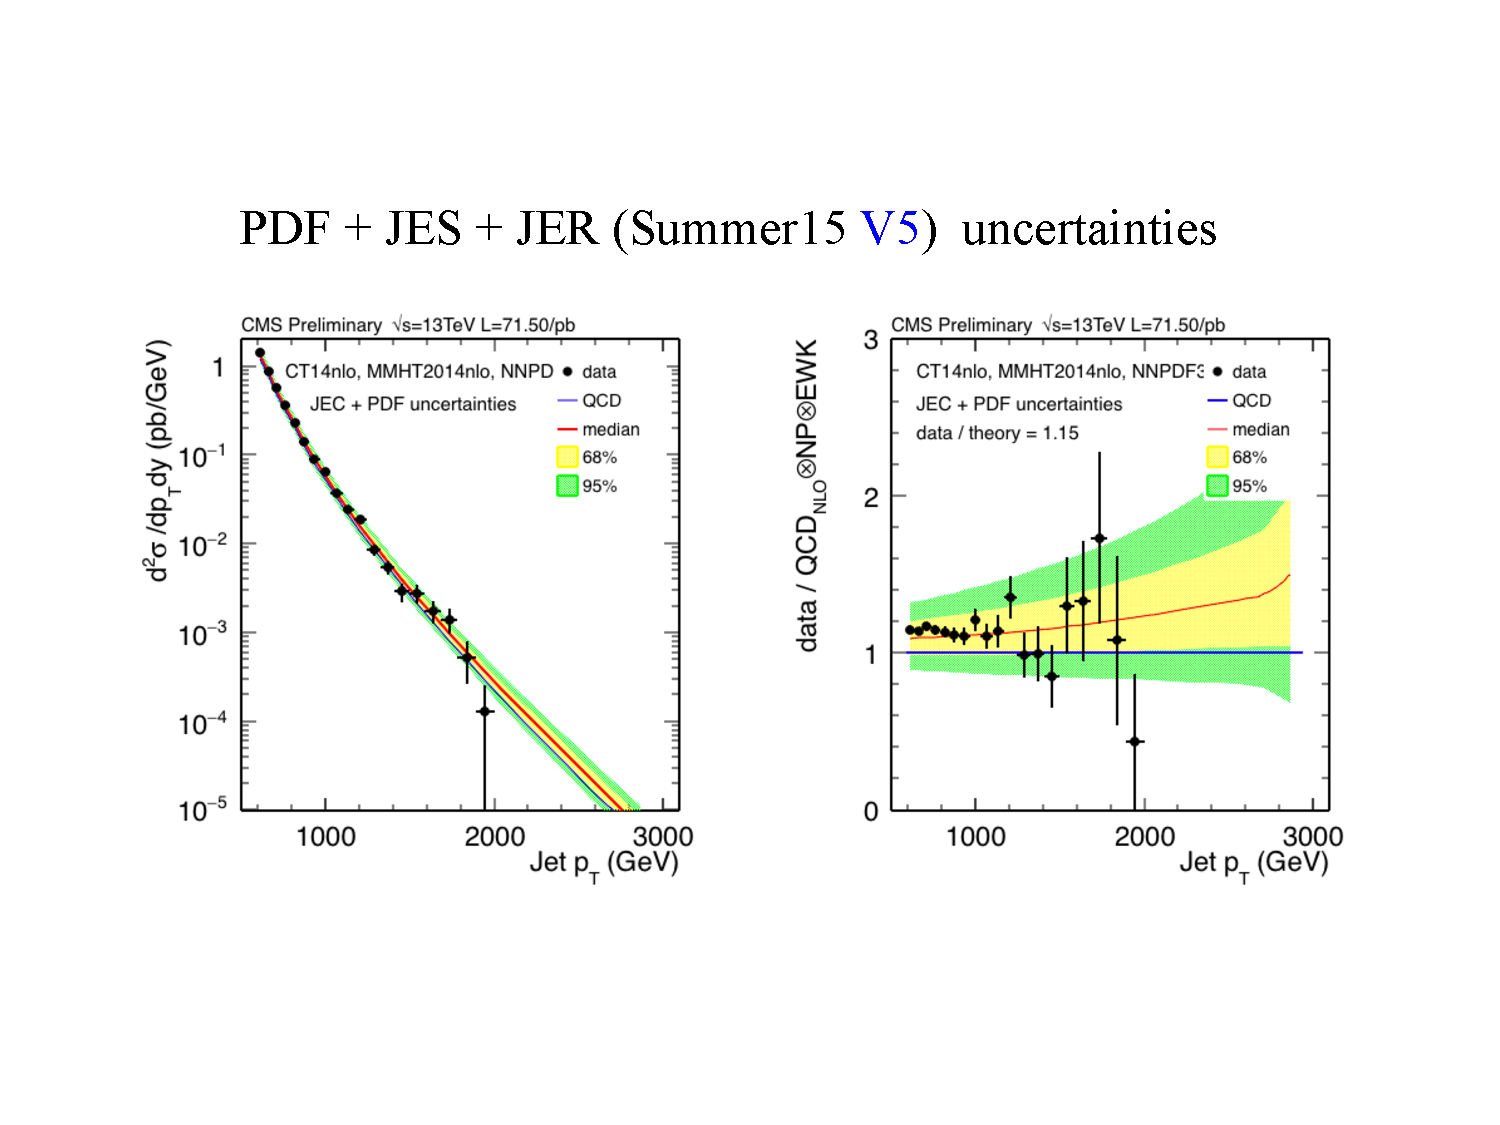
\includegraphics[width=\textwidth]{fig_data_QCD.pdf}
}
\end{frame}

\begin{frame}
\centerline{
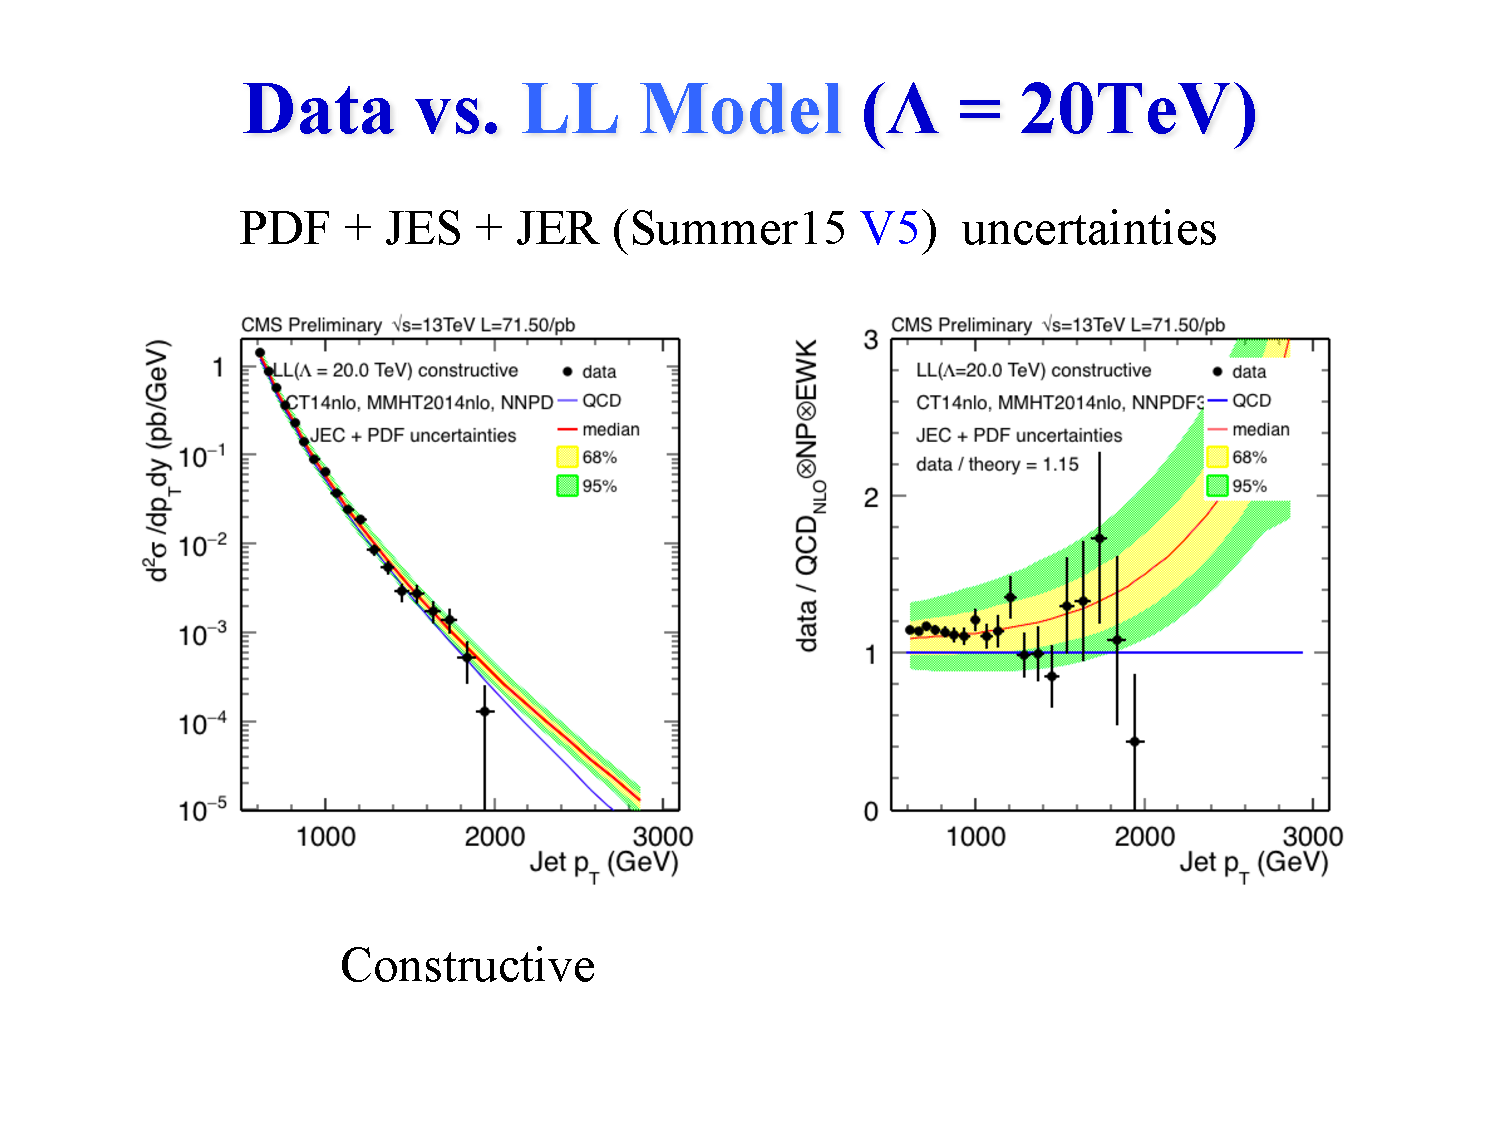
\includegraphics[width=\textwidth]{fig_data_LL.pdf}
}
\end{frame}


\begin{frame}
\centerline{
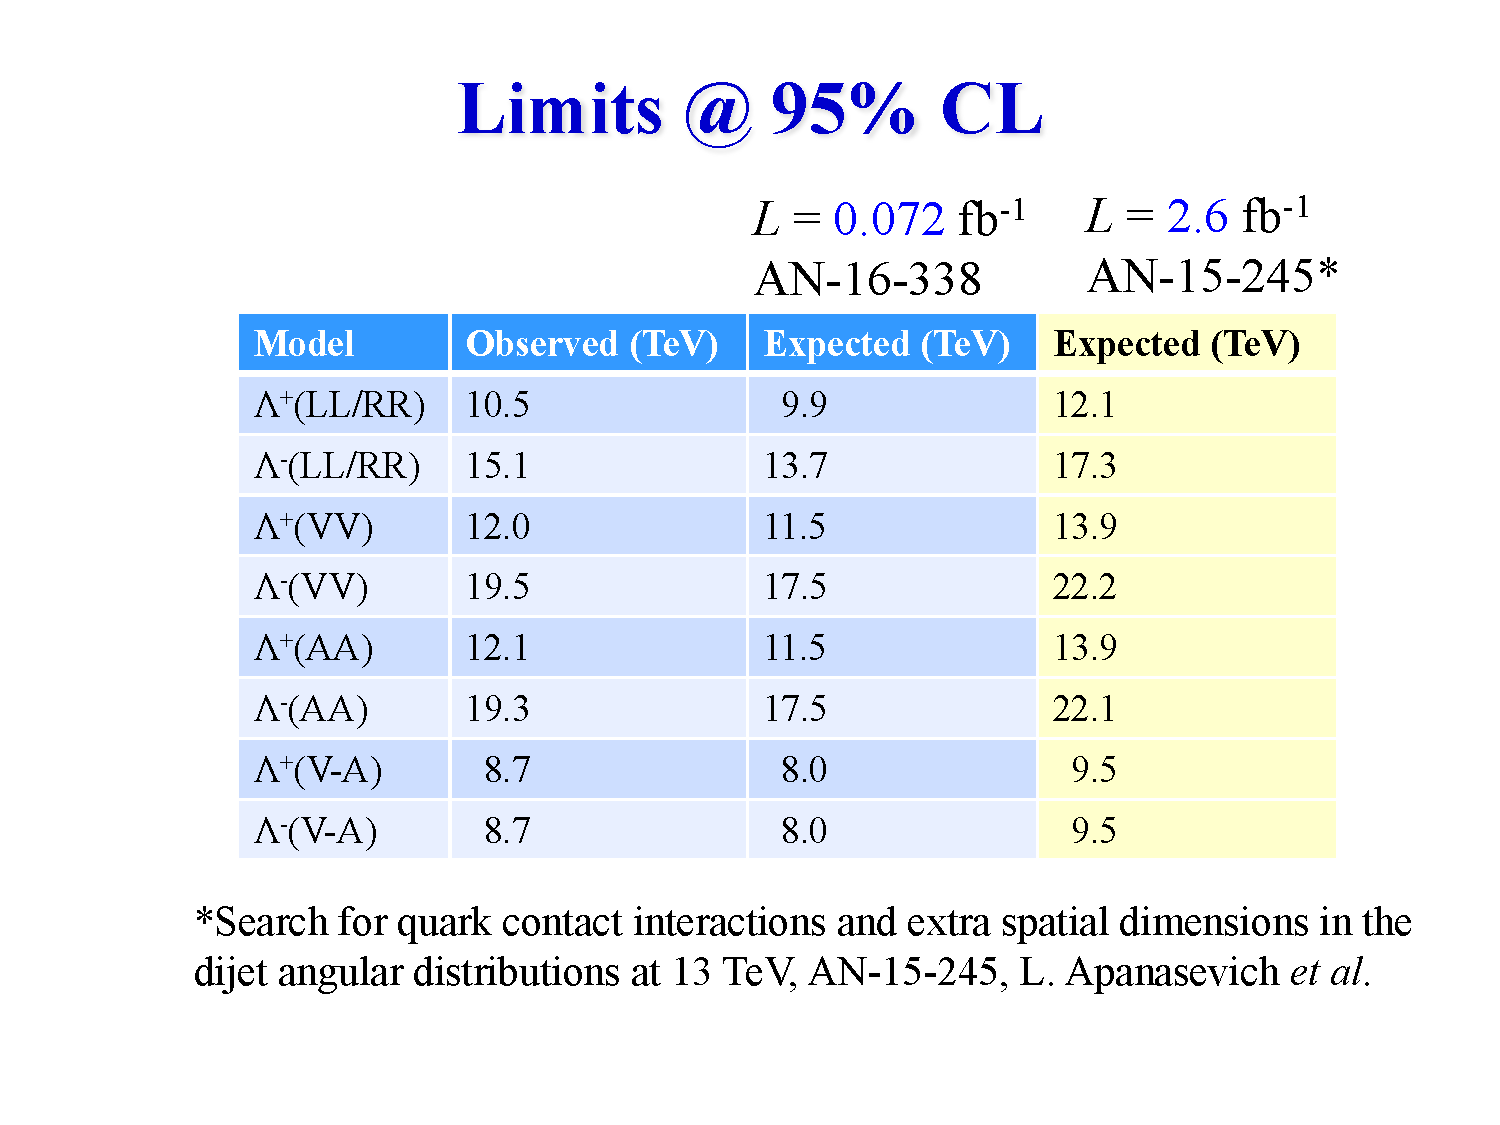
\includegraphics[width=\textwidth]{fig_results.pdf}
}
\end{frame}


\begin{frame}
\centerline{
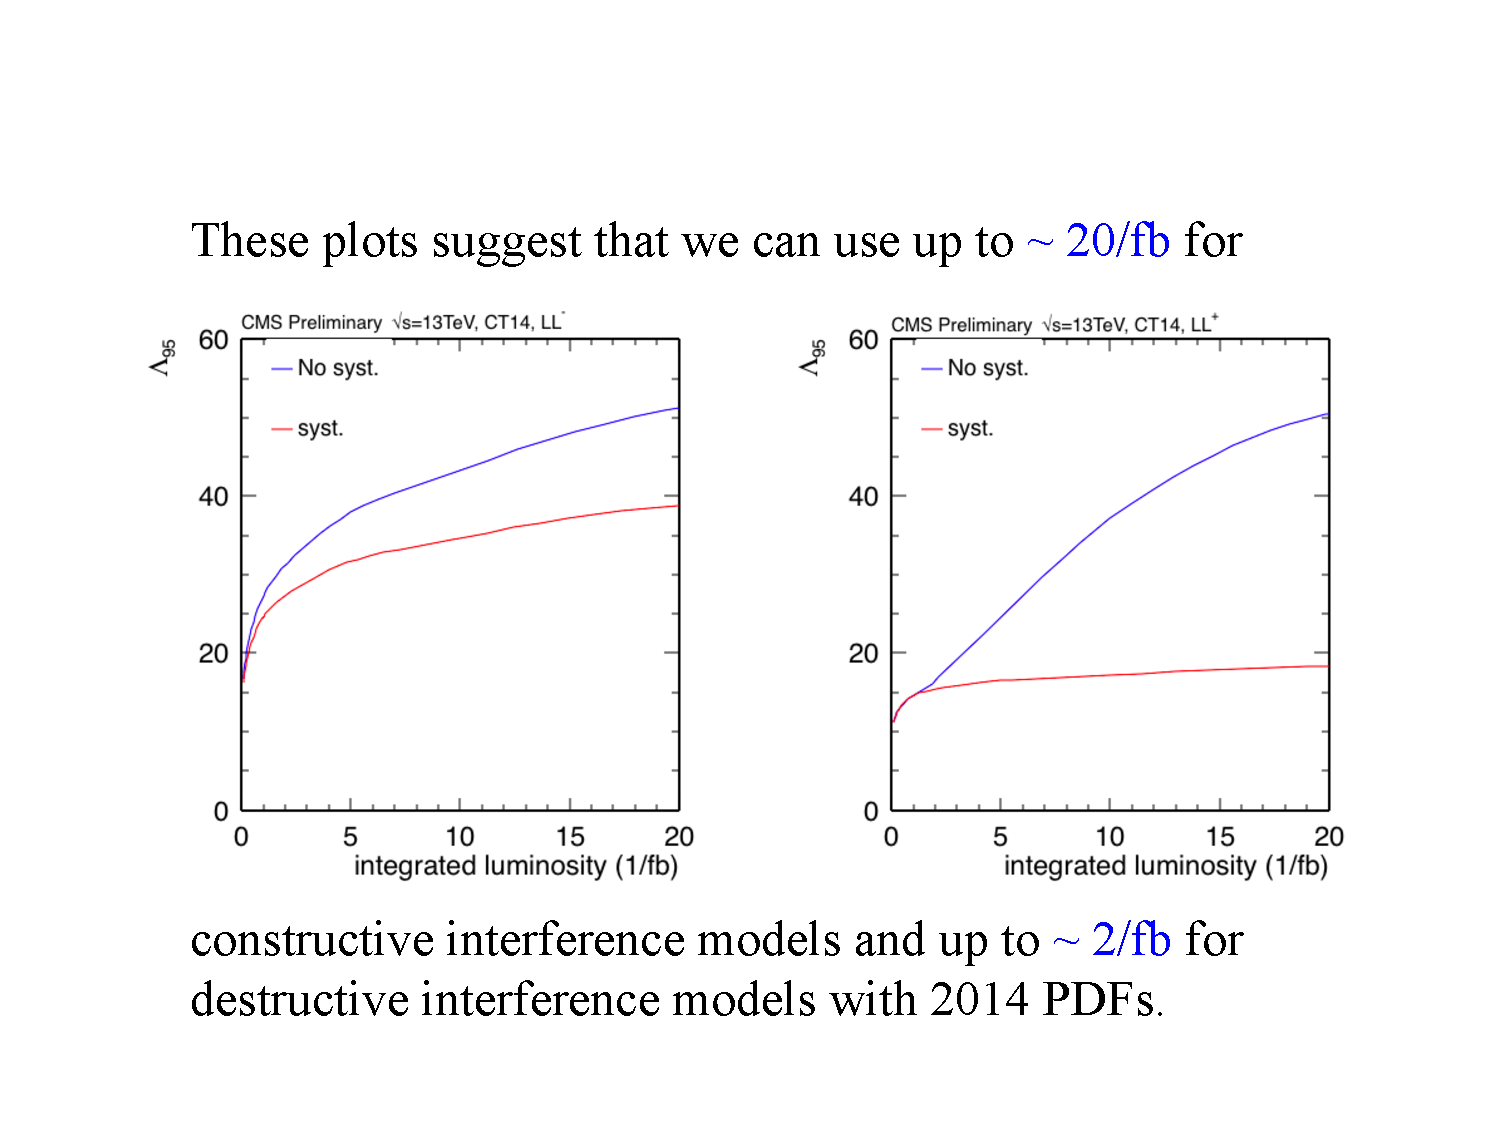
\includegraphics[width=\textwidth]{fig_projections.pdf}
}
\end{frame}

\begin{frame}
\begin{columns}[T]
\begin{column}{0.35\textwidth}
\textcolor{blue}{Pileup Studies} The plot, based on 
$2.6\,\textrm{fb}^{-1}$, show ratios of the AK7 jet $p_\textrm{T}$ spectra
in different vertex multiplicity bins for jets with $|y| < 0.5, p_{\textrm{T}} > 600\,\textrm{GeV}$.
The data are collected with the Jet450 trigger. The binning is uniform.
\end{column}
\begin{column}{0.65\textwidth}
\centerline{
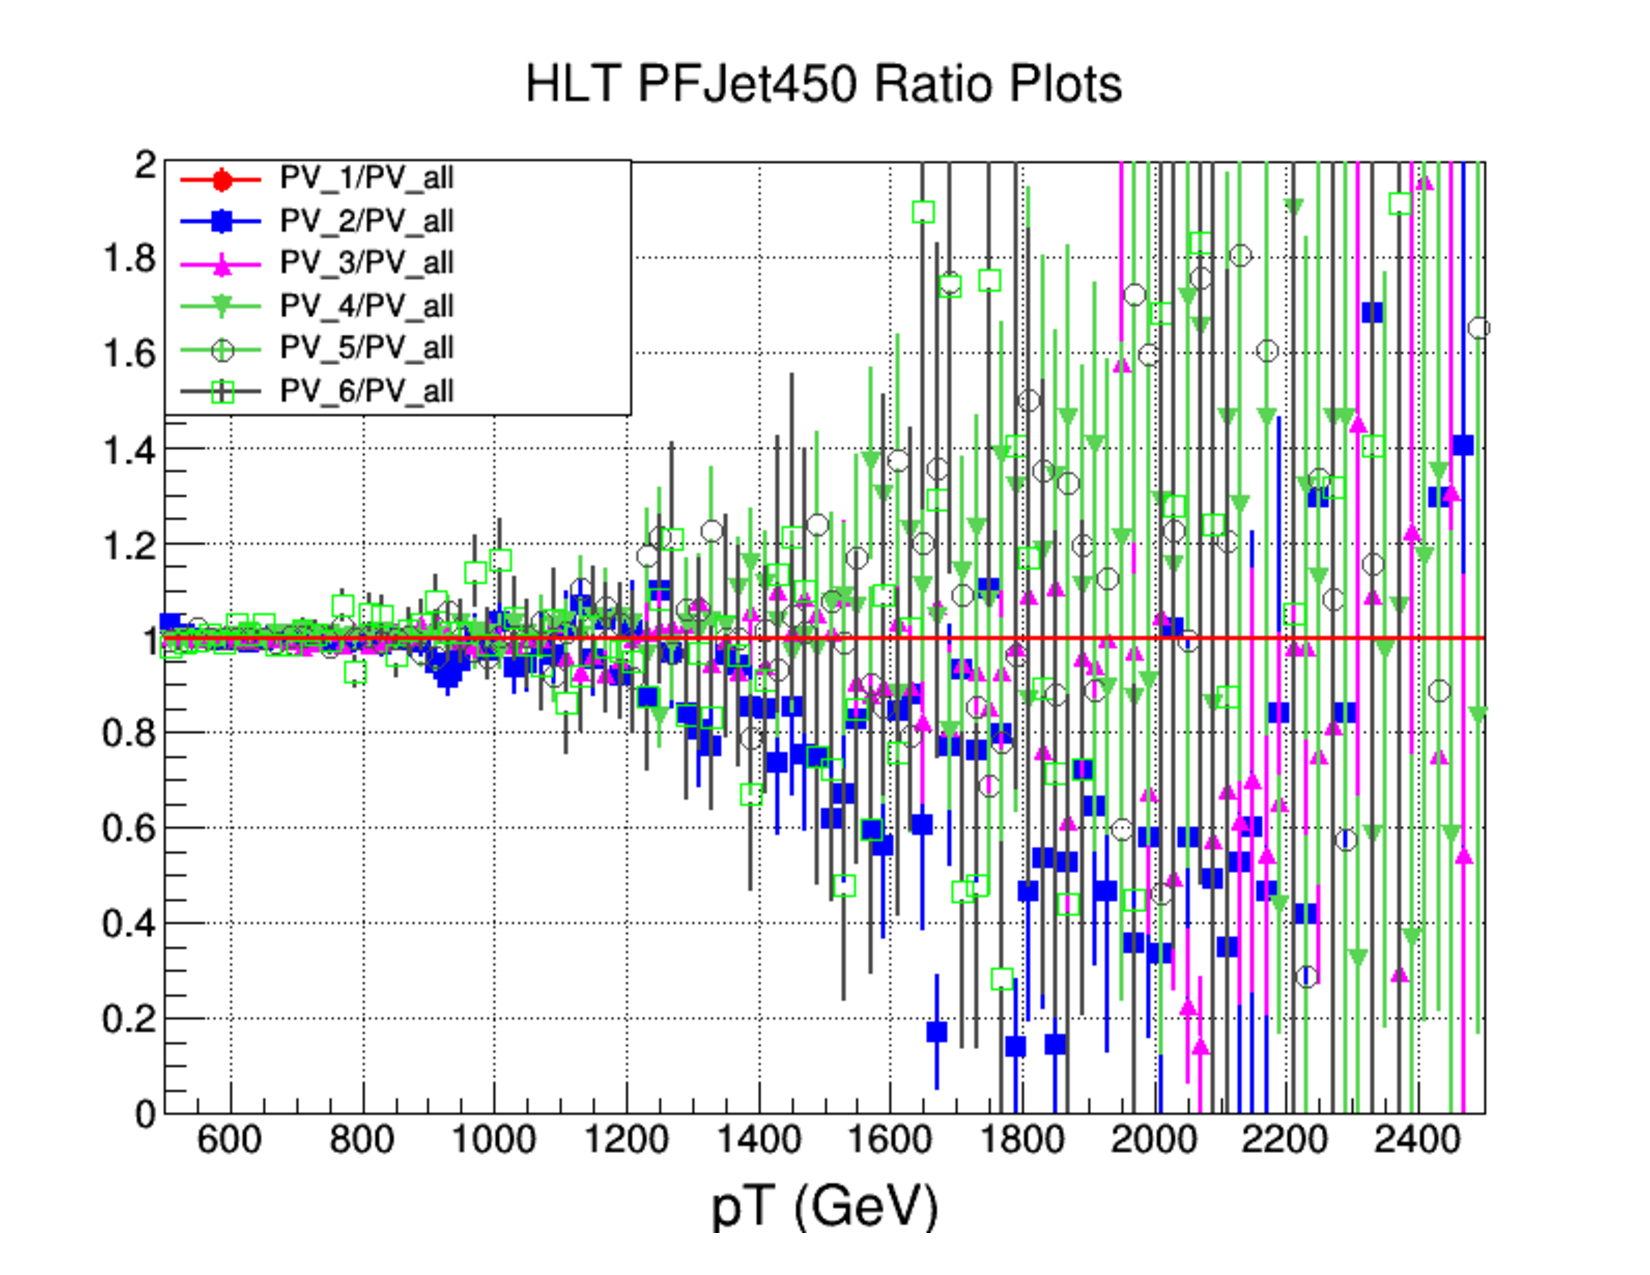
\includegraphics[width=\textwidth]{RatioJet450.pdf}
}
\end{column}
\end{columns}
\end{frame}

\section{Near Term Plans}
\begin{frame}
\textcolor{blue}{Near Term Plans ($\sim$ 2 weeks)}
\begin{itemize}
\item Compute preliminary \emph{expected} limits for models defined by different combinations of $\bkappa$.
Use the existing QCD cross sections computed with
\textcolor{blue}{\tt fastnlo\_toolkit-2.3.1pre-1871} and \textcolor{blue}{\tt InclusiveNjets\_fnl5332g\_v23\_fix.tab},
and the CI coefficients computed with \textcolor{blue}{\tt CIJet-1.1}. For now, do this only for \textcolor{blue}{\tt CT14nlo}.
\item Update our smearing code to use the current JES and JER
functions and NP and EWK corrections. 
\item To proceed, we  need:
\begin{itemize}
	\item observed jet counts for all bins above $\sim 600\,\textrm{GeV}$;
	\item non-perturbative correction histogram;
	\item electroweak correction histogram, and
	\item detailed description of current JES and JER functions.
\end{itemize}
\end{itemize}
\end{frame}



\end{document}